%%%%%%%%%%%%%%%%%%%%%%%%%%%%%%%%%%%%%%%%%
% Beamer Presentation
% LaTeX Template
% Version 1.0 (10/11/12)
%
% This template has been downloaded from:
% http://www.LaTeXTemplates.com
%
% License:
% CC BY-NC-SA 3.0 (http://creativecommons.org/licenses/by-nc-sa/3.0/)
%
%%%%%%%%%%%%%%%%%%%%%%%%%%%%%%%%%%%%%%%%%

%----------------------------------------------------------------------------------------
%	PACKAGES AND THEMES
%----------------------------------------------------------------------------------------

\documentclass{beamer}
\usepackage[T1]{fontenc}
\usepackage{lmodern}
\usepackage[utf8]{inputenc}
\usepackage[german]{babel}
\usepackage[11pt]{moresize}


\mode<presentation> {

% The Beamer class comes with a number of default slide themes
% which change the colors and layouts of slides. Below this is a list
% of all the themes, uncomment each in turn to see what they look like.

%\usetheme{default}
%\usetheme{AnnArbor}
%\usetheme{Antibes}
%\usetheme{Bergen}
%\usetheme{Berkeley}
\usetheme{Berlin}
%\usetheme{Boadilla}
%\usetheme{CambridgeUS}
%\usetheme{Copenhagen}
%\usetheme{Darmstadt}
%\usetheme{Dresden}
%\usetheme{Frankfurt}
%\usetheme{Goettingen}
%\usetheme{Hannover}
%\usetheme{Ilmenau}
%\usetheme{JuanLesPins}
%\usetheme{Luebeck}
%\usetheme{Madrid}
%\usetheme{Malmoe}
%\usetheme{Marburg}
%\usetheme{Montpellier}
%\usetheme{PaloAlto}
%\usetheme{Pittsburgh}
%\usetheme{Rochester}
%\usetheme{Singapore}
%\usetheme{Szeged}
%\usetheme{Warsaw}

% As well as themes, the Beamer class has a number of color themes
% for any slide theme. Uncomment each of these in turn to see how it
% changes the colors of your current slide theme.

%\usecolortheme{albatross}
%\usecolortheme{beaver}
%\usecolortheme{beetle}
%\usecolortheme{crane}
%\usecolortheme{dolphin}
%\usecolortheme{dove}
%\usecolortheme{fly}
%\usecolortheme{lily}
%\usecolortheme{orchid}
%\usecolortheme{rose}
%\usecolortheme{seagull}
%\usecolortheme{seahorse}
%\usecolortheme{whale}
%\usecolortheme{wolverine}

%\setbeamertemplate{footline} % To remove the footer line in all slides uncomment this line
%\setbeamertemplate{footline}[page number] % To replace the footer line in all slides with a simple slide count uncomment this line

%\setbeamertemplate{navigation symbols}{} % To remove the navigation symbols from the bottom of all slides uncomment this line
}

\usepackage{graphicx} % Allows including images
\usepackage{booktabs} % Allows the use of \toprule, \midrule and \bottomrule in tables

%----------------------------------------------------------------------------------------
%	TITLE PAGE
%----------------------------------------------------------------------------------------

\title[Definitionsphase]{Kolloqium Definitionsphase} % The short title appears at the bottom of every slide, the full title is only on the title page

\author{Phasenverantwortliche: Chiara Staudenmaier} % Your name
\institute[PSE] % Your institution as it will appear on the bottom of every slide, may be shorthand to save space
{

}
\date{\today} % Date, can be changed to a custom date

\begin{document}

\begin{frame}
\titlepage % Print the title page as the first slide
\end{frame}

%\begin{frame}
%\frametitle{Overview} % Table of contents slide, comment this block out to remove it
%\tableofcontents % Throughout your presentation, if you choose to use \section{} and \subsection{} commands, these will automatically be printed on this slide as an overview of your presentation
%\end{frame}

%----------------------------------------------------------------------------------------
%	PRESENTATION SLIDES
%----------------------------------------------------------------------------------------

%------------------------------------------------
\section{Produktübersicht} % Sections can be created in order to organize your presentation into discrete blocks, all sections and subsections are automatically printed in the table of contents as an overview of the talk
%------------------------------------------------

\subsection{Produktübersicht} % A subsection can be created just before a set of slides with a common theme to further break down your presentation into chunks

\begin{frame}
\frametitle{DIbugger}

\includegraphics[scale=0.3]{../logo_nongi}
\end{frame}

\section{Sprache}
\subsection{Sprache}
\subsubsection{Sprache}
\begin{frame}
\frametitle{Elemente der Sprache}
\begin{itemize}
\item  32-bit Ganzzahlen: \texttt{int}
  \item  64-bit Ganzzahlen: \texttt{long}
 \item  32-bit IEEE 754 Fließkommazahlen: \texttt{float}
 \item   64-bit IEEE 754 Fließkommazahlen: \texttt{double}
  \item  Einzelnes Zeichen: \texttt{char}
  \item  Wahrheitswert: \texttt{boolean}
\item Funktionen und Prozeduren % Unterprogramme mit oder ohne Rückgabewert.
\item Bedingte Ausführung: \texttt{if, else if, else}
\item Schleifen: \texttt{while}
\end{itemize}
\end{frame}


%------------------------------------------------
\subsection{Produkteinsatz}
\begin{frame}
\frametitle{Produkteinsatz}
\end{frame}

%------------------------------------------------
\subsection{Produktumgebung}
\begin{frame}
\frametitle{Produktumgebung}
\begin{itemize}
\item Software
\item Hardware
\item Schnittstellen
\end{itemize}
\end{frame}

%------------------------------------------------

\section{Produktfunktionen}
\subsection{Funktionale Anforderungen}
\begin{frame}
\frametitle{Musskriterien}
\end{frame}

%------------------------------------------------
\subsubsection{Sollkriterien}
\begin{frame}
\frametitle{Sollkriterien}
\end{frame}

%------------------------------------------------
\subsubsection{Kannkriterien}
\begin{frame}
\frametitle{Kannkriterien}
\end{frame}
%-----------------------------------------------
\subsubsection{Abgrenzungskriterien}
\begin{frame}
\frametitle{Abgrenzungskriterien}
\end{frame}

%----------------------------------------------

\subsection{Nichtfunktionale Anforderungen}
\subsubsection{Produktdaten}
\begin{frame}
\frametitle{Produktdaten}
\begin{itemize}
\item Konfigurationsdateien
\item Sprachdateien
\item Einstellungsdatei
\end{itemize}
\end{frame}
%---------------------------------------------
\subsubsection{Produktleistungen}
\begin{frame}
\frametitle{Produktleistungen}
\begin{itemize}
\item Zeitverhalten
\item Genauigkeit
\item Fehlertoleranz
\end{itemize}
\end{frame}
%-------------------------------------------
\subsubsection{Weitere nichtfunktionale Anforderungen}
\begin{frame}
\frametitle{Weitere nichtfunktionale Anforderungen}
\begin{itemize}
\item Erweiterbarkeit
\item Wartbarkeit
\item Urheberrecht
\item Sicherheit
\item Benutzerfreundlichkeit
\end{itemize}
\end{frame}


\section{Testfälle und Anwendungsfälle}

%------------------------------------------------
\subsection{Anwendungsfälle}
\begin{frame}
\frametitle{Anwendungsfälle}
\end{frame}

%------------------------------------------------
\section{Qualitätsanforderungen}
\subsection{Qualitätsanforderungen}
\begin{frame}
\frametitle{Qualitätsanforderungen}
\begin{ssmall}
\begin{tabular}{l||l|c|c|c|c} 
    & Produktqualität & Sehr gut & Gut & Normal & Nicht relevant \\
  \hline
  \hline
  \textbf{Funktionalität} &Angemessenheit & & & X &  \\
  %\cline{2-6}
  &Richtigkeit & X & & & \\
  %\cline{2-6}
  &Interoperabilität & & & X &\\
  %\cline{2-6}
  &Sicherheit & & & X & \\
  \hline
  \textbf{Zuverlässigkeit} &Reife & & & X & \\
  %\cline{2-6}
  &Fehlertoleranz & & & X & \\
  %\cline{2-6}
  &Wiederherstellbarkeit & & & X &\\
  \hline
  \textbf{Benutzbarkeit} &Verständlichkeit & & X & &\\
  %\cline{2-6}
  &Erlernbarkeit & & X & &\\
  %\cline{2-6}
  &Bedienbarkeit & X & & &\\
  \hline
  \textbf{Effizienz} &Zeitverhalten & & & X & \\
  %\cline{2-6}
  &Verbauchsverhalten & & & X & \\
  \hline
  \textbf{Änderbarkeit} &Analysierbarkeit & & & X &\\
  %\cline{2-6}
  &Modifizierbarkeit & X & & &\\
  %\cline{2-6}
  &Stabilität & & X&  &\\
  %\cline{2-6}
  &Prüfbarkeit & & & X &\\
  \hline
  \textbf{Übertragbarkeit} &Anpassbarkeit & & X & &\\
  %\cline{2-6}
  &Installierbarkeit & & X & & \\
  %\cline{2-6}
  &Konformität & & & X & \\
  %\cline{2-6}
  &Austauschbarkeit & & & X & \\
 \end{tabular}
 \end{ssmall}
\end{frame}

%------------------------------------------------
\subsection{Globale Testfälle}
\begin{frame}
\frametitle{Globale Testfälle}
\end{frame}

%------------------------------------------------
\section{Systemmodelle}
\subsection{Aktivitätsdiagramm}
\begin{frame}
\frametitle{Aktivitätsdiagramm}
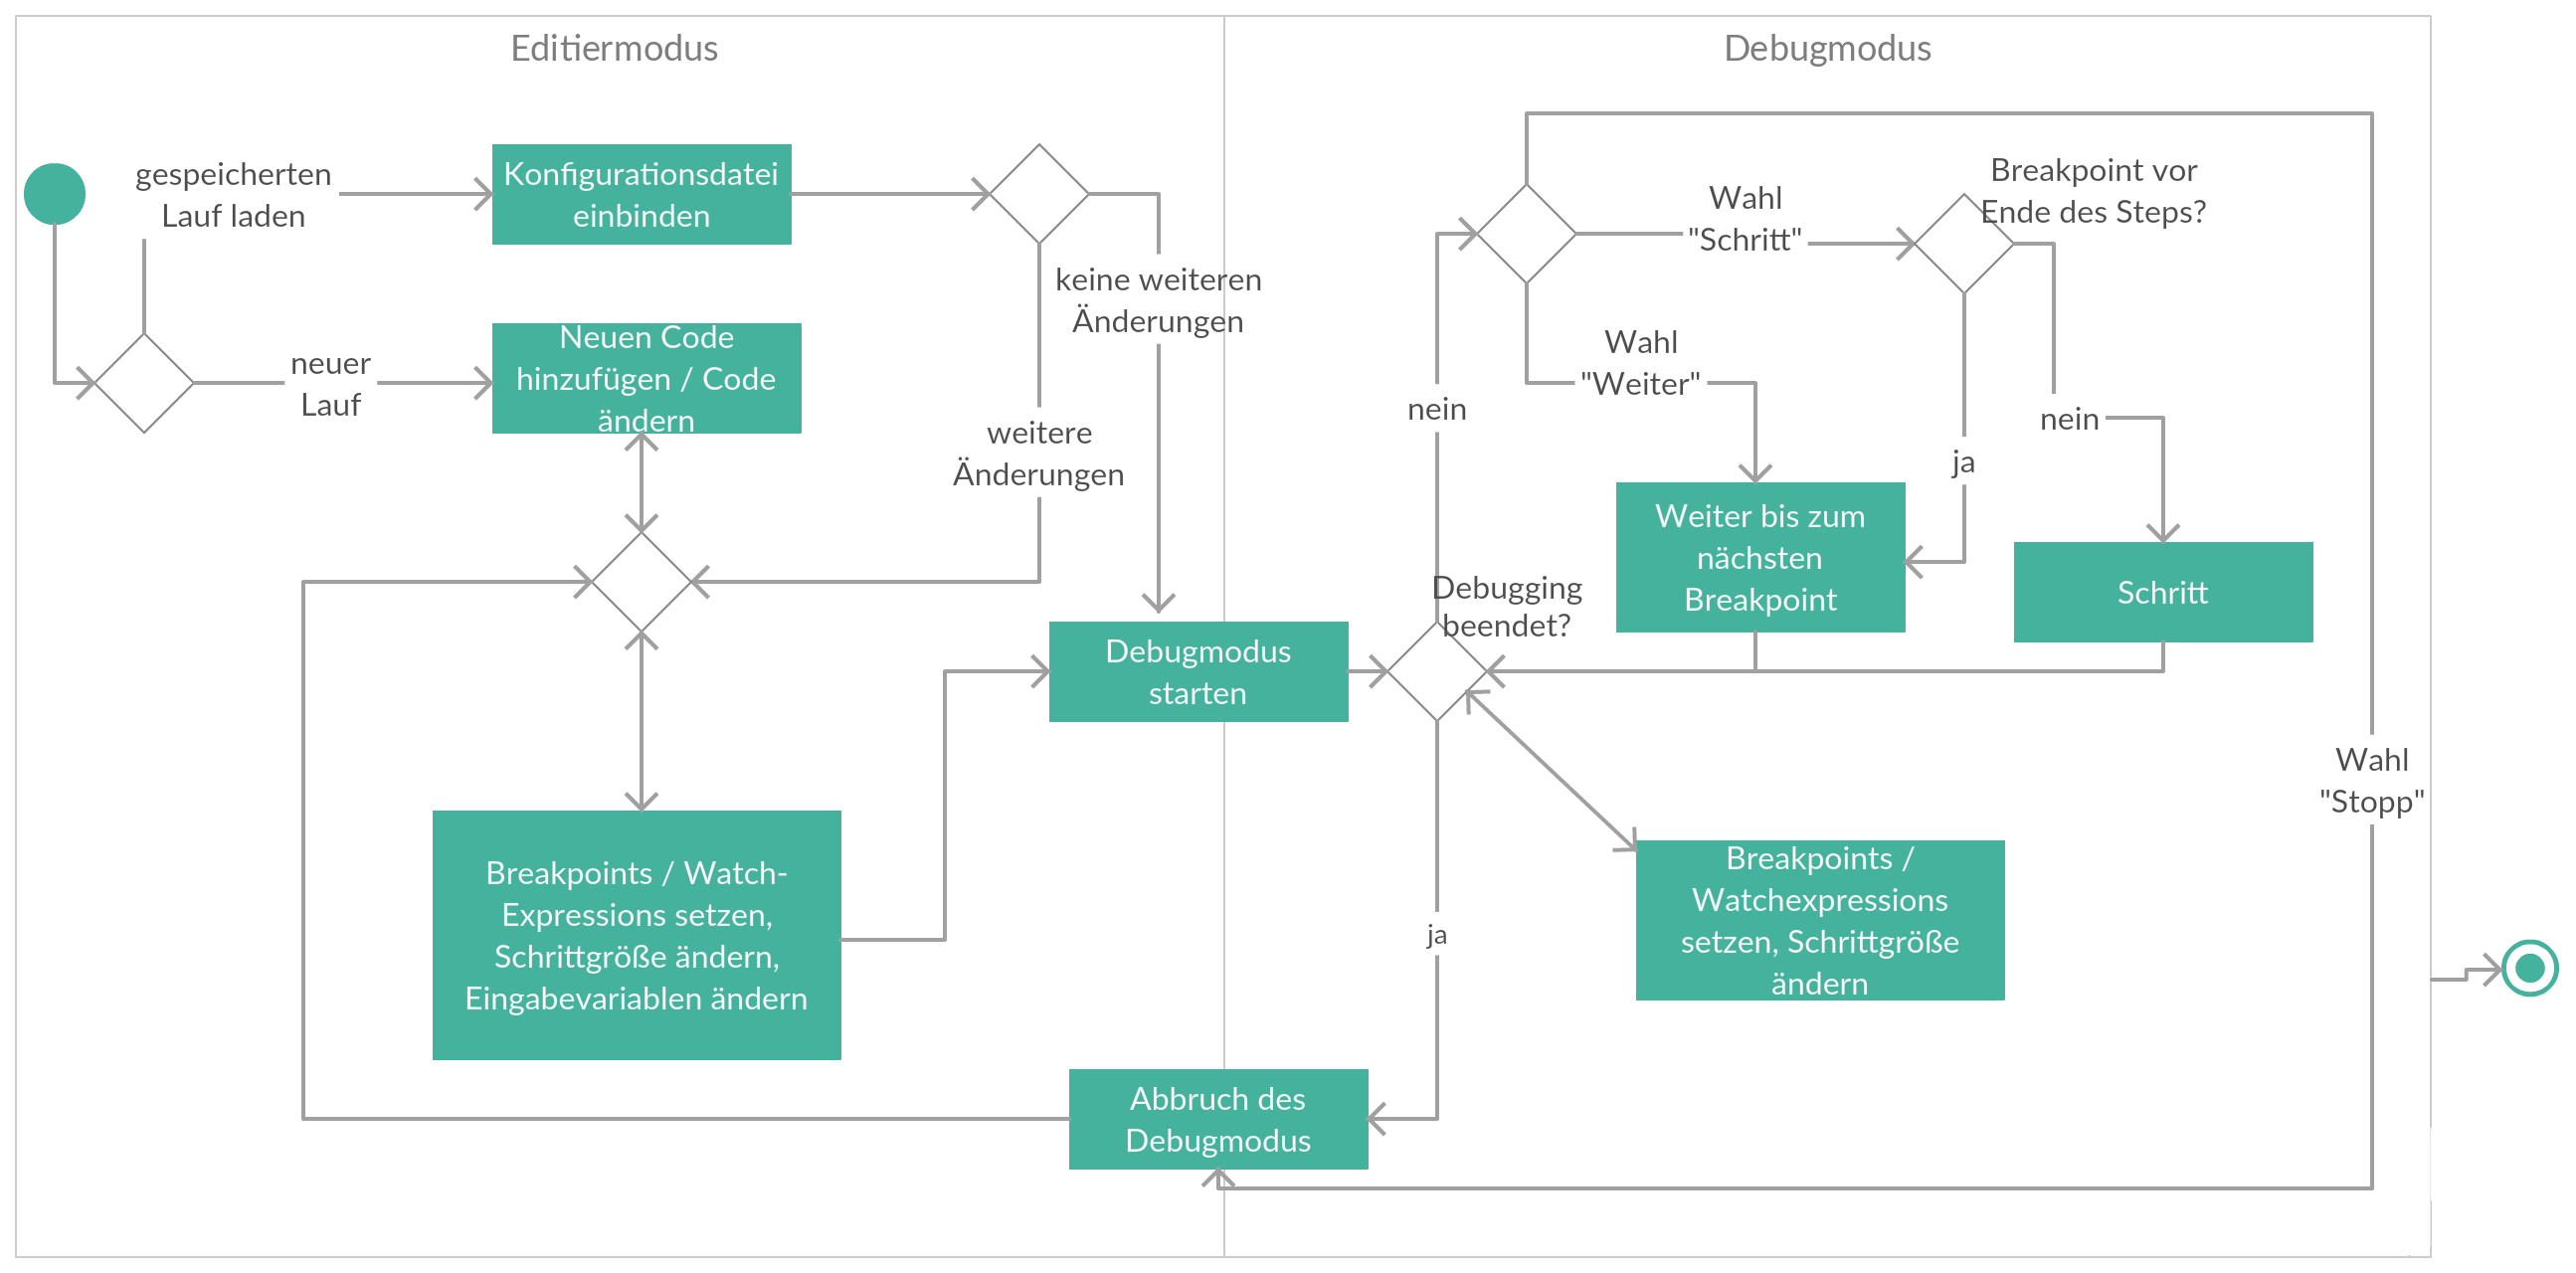
\includegraphics[scale=0.12]{../Aktivitaetsdiagramm}
\end{frame}


%------------------------------------------------
\section{GUI}
\subsection{Editiermodus}
\begin{frame}
\frametitle{Editiermodus}
%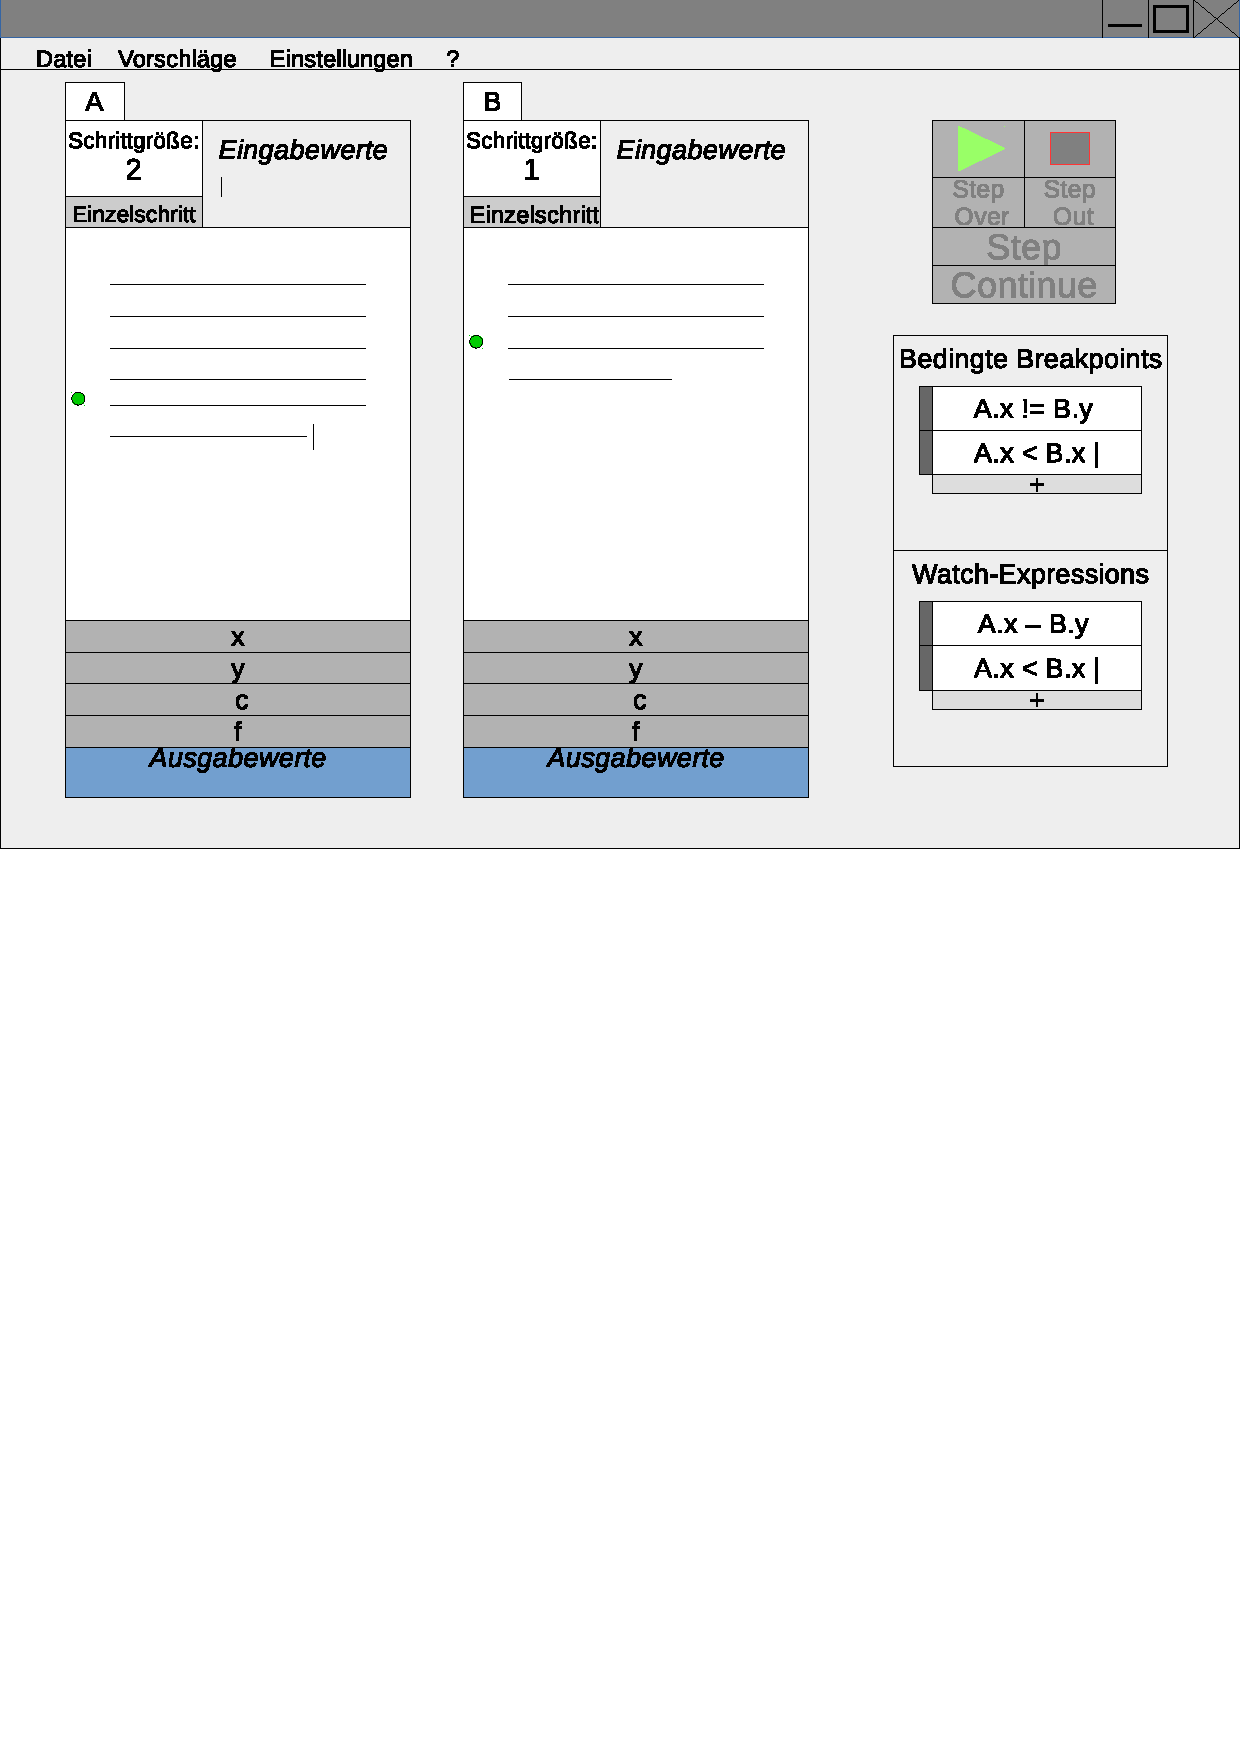
\includegraphics[scale=0.45]{../skizzeEdit}
\end{frame}

\subsection{Debugmodus}
\begin{frame}
\frametitle{Debugmodus}
%\includegraphics[scale=0.5]{../skizzeDebug.eps}
\end{frame}

%------------------------------------------------


%----------------------------------------------------------------------------------------

\end{document} 